% Chapter Template

\chapter{Summary of Previous Work} % Main chapter title

\label{Chapter2} 

\lhead{Chapter 2. \emph{Summary of Previous Work}} 

Response matrix methods have traditionally used a full multigroup 
representation of the energy variable, which is to say that there is no basis 
truncation for the energy basis.  Response matrix methods have been used 
successfully with a variety of energy group structures, ranging from three to 
190 groups \citep{ishii2009tdd, forget2006tdh, forget2004hcm}. 

One of the first studies of a truncated energy expansion for response matrix 
methods was the work of \citet{Roberts2014}, who used Discrete 
Legendre Polynomials (DLP) and a modified version of DLP (mDLP) to expand in 
energy. His approach compared the basis expansions to a full multigroup 
approximation of the energy variable.  

This chapter aims to explore the previous work in expanding the energy 
variable, beginning with a brief overview of how the full multigroup approach 
can be represented in the formalism of \CHAPTER{Chapter1}, followed by a 
discussion 
of DLPs and problem-specific, modified DLPs.

%-------------------------------------------------------------------------------

\section{Expanding in Energy}

In order to represent the multigroup method exactly in ERMM, the energy 
variable is represented by a set of Kronecker-$\delta$ functions defined by
\begin{equation}
  P_{\delta}^h(g) = \delta_{h, g-1},\, g=1,\, 2, \, \ldots,\, G \, ,
\end{equation}
where 
\begin{equation}
    \delta_{h, g-1} = 
    \begin{cases}
        1, & \text{if }  h = g-1 \, , \\
        0, & \text{if }  h \neq g-1 \, .
    \end{cases}
\end{equation}

When a complete set  of these vectors (i.e., $H = G-1$) is used, a generic 
response function moment $R^{s'l'h' \to slh}$ can be rewritten as $R^{s'l'g' \to 
slg}$.  Thus, the group-to-group transfer process is represented in the 
traditional form.  However, this approach requires that 
all energy groups be included, thus the number of energy degrees of freedom is 
equal to the number of groups.  This method works well when the number of groups 
is low, but large models become prohibitively expensive when a detailed energy 
treatment (i.e., more than approximately 10 groups) is used. 

If a Kronecker set is truncated, a significant amount of the physics is lost, 
and the expansion has significantly reduced accuracy. Hence, the Kronecker set 
should not be used with energy order reduction. In order to improve ERMM 
performance, a basis set for energy is sought that will capture many-group 
fidelity while requiring many fewer degrees of freedom ($H$ in 
\EQSTWO{eq:finalfluxmoments}{eq:finalcurrentmoments}) than a full 
multigroup analysis (a solution utilizing the complete set of Kronecker 
vectors).

A way to reduce the energy degrees of freedom is to use an orthogonal basis to 
approximate the functionality of every group, thus converting the energy degrees 
of freedom
for the problem into the coefficients of expansion. In this case, the energy 
degrees of freedom are equal in number to $G$, because $H+1$ basis functions 
are required to expand exactly a vector of length $G$.  The problem is then 
simplified by using a lower expansion order than $G$.  If the low-order 
vectors in a basis set can better approximate the energy dependence, then the 
truncation should minimize effect of the error introduced such an expansion.  
The previous work by \citet{Roberts2014} suggested that incorporating physics 
directly into the basis functions may be more efficient than standard basis 
sets, and can lead to accuracy close to that of a 
full multigroup treatment using $G$ groups without needing $H+1$ energy degrees 
of freedom.

Each of the basis sets presented here are computed in orthonormal 
form.  This formulation leads to quick determination of the expansion 
coefficients similarly to 
\EQSTWO{eq:groupcoefficients}{eq:groupcurrentcoefficients}, rewritten as
\begin{equation}
    a_i = \sum_{g=0}^{G}w(g) P^i(g) f(g) \, ,
  \label{eq:coefficients}
\end{equation}
where $a_i$ is the $i$th coefficient of expansion, $w(g)$ is the weight 
associated with the basis function, $P^i(g)$ is the $i$th basis function, and
$f(g)$ 
is the function to expand. The 
reconstructed function is given by
\begin{equation}
    \tilde{f}(g) \approx \sum_{i=0}^{I} a_i P^i(g)
  \label{eq:expansion}
\end{equation}
where $I$ is the expansion order.  

\EQUATION{eq:expansion} is defined akin to 
\EQSTWO{eq:groupfluxmoments}{eq:groupcurrentmoments}. Because a 
reduced number of energy degrees of freedom is desired, a basis that 
incorporates some physics of the problem is likely to provide the best 
expansion.  The basis that includes physics should then be compared to more 
standard basis sets, such as the Discrete Legendre Polynomials (DLPs).

%-------------------------------------------------------------------------------

\section{Discrete Legendre Polynomials}

The Legendre polynomials form a standard and proven basis that is used 
throughout computational physics.  The discrete versions of the Legendre 
polynomials are shown in \FIG{fig:DLP}.  When using the DLPs, the 
functions are represented by vectors of length equal to the number of 
discretized points.  The vectors shown in \FIG{fig:DLP} have been 
orthonormalized over the range of the vectors. Recent work 
investigated the use of discrete Legendre polynomials (DLPs) for expansion in 
energy \citep{Roberts2014, Zhu2010, Zhu2011}.  The set of polynomials is 
generated using the 
Gram-Schmidt process to orthogonalize the discrete monomials $M^h(g) =  g^h,\, 
g=0,\,1,\,\ldots,\, G-1$. To illustrate, let $G=5$, for which the zeroth-order 
DLP vector is defined as
\begin{equation}
    \begin{split}
        P_{\text{DLP}}^0(:) &= \frac{M^0(:)}{\sqrt{\sum_{g=1}^{G} M^0(g)}} \\
        &= \frac{\sqrt{5}}{5}[1,\,1,\,1,\,1,\,1]^{\intercal} \, .
    \end{split}
\end{equation}
To define the  first-order DLP vector, let
\begin{equation}
    \begin{split}
        \tilde{P}_{\text{DLP}}^1(:) &= M^1(:) - \left ( \sum_{g=1}^{G} 
        P_{\text{DLP}}^0(g) M^1(g) \right ) P_{\text{DLP}}^0(:)   \, ,
        %          &=  \frac{1}{2}[-3,\,-1,\,1,\,3]^{\intercal} \, ,
    \end{split}
\end{equation}
leading to
\begin{equation}
    \begin{split}
        P_{\text{DLP}}^1(:) &= 
        \frac{\tilde{P}_{\text{DLP}}^1(:)}{\sqrt{\sum_{g=1}^{G} 
                \tilde{P}_{\text{DLP}}^1(g)\tilde{P}_{\text{DLP}}^1(g)}} \\
        &= \frac{\sqrt{10}}{5} [-2,\,-1,\,0,\,1,\,2]^{\intercal} \, .
    \end{split}
\end{equation}

\begin{figure*}[pt]
  \centering
  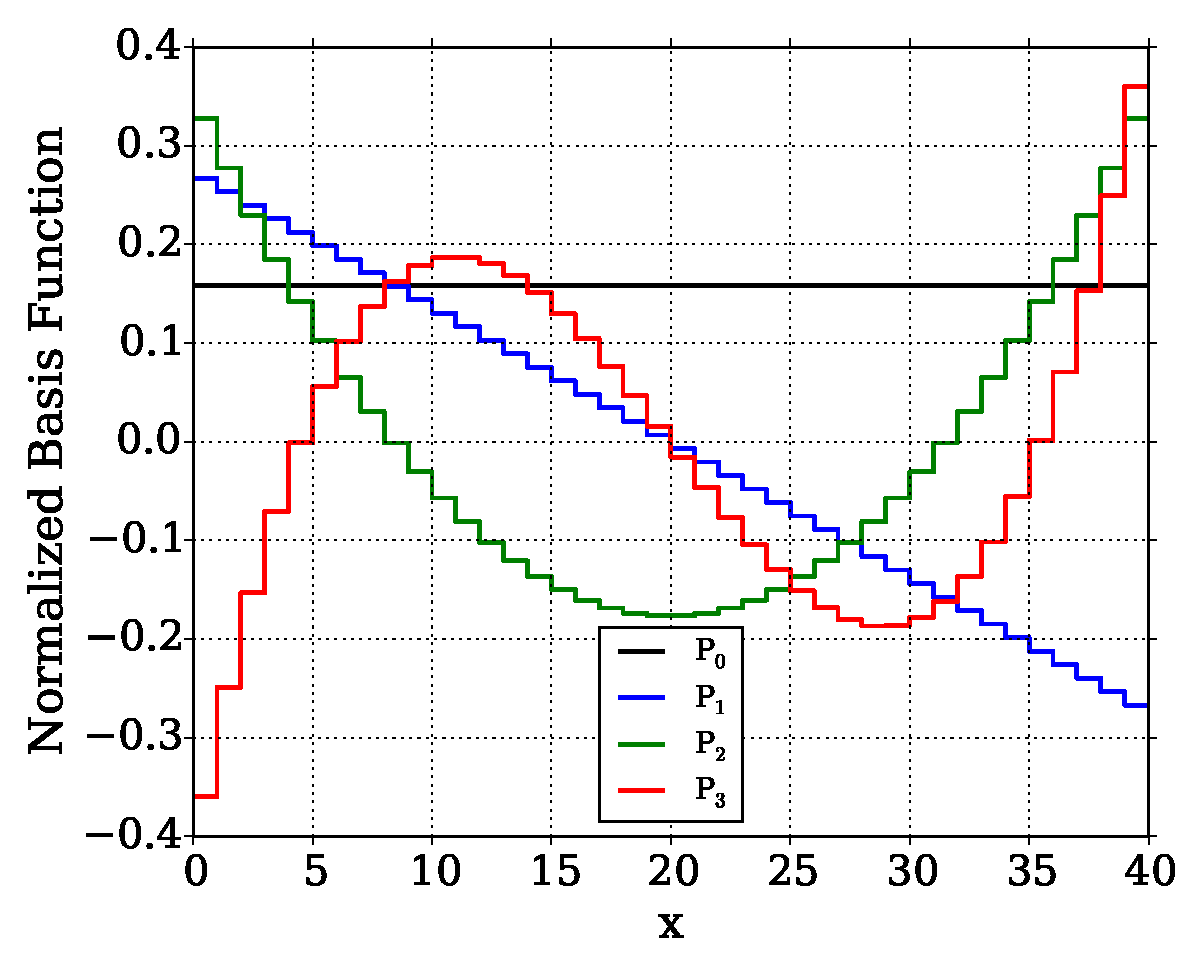
\includegraphics[trim=.1cm .25cm .1cm .4cm, clip=true,
  totalheight=0.35\textheight]{Figures/DLP_basis}
  \caption{Discrete Legendre Polynomials shown through $3^{rd}$ order using 40 
points}
  \label{fig:DLP}
\end{figure*}

This procedure can be repeated for DLP vectors of arbitrary order, up through 
one less than number of energy groups used. For the provided example, the 
second-, third-, and 
fourth-order DLP vectors are defined as
\begin{equation}
    \begin{split}
        P_{\text{DLP}}^2(:)  &= \frac{\sqrt{146}}{146} 
        [8,\,-1,\,-4,\,-1,\,8]^{\intercal} \\
        P_{\text{DLP}}^3(:)  &= \frac{\sqrt{610}}{610} 
        [-16,\,7,\,0,\,-7,\,16]^{\intercal} \\
        P_{\text{DLP}}^4(:)  &= \frac{\sqrt{1090}}{5450} 
        [80,\,-85,\,0,\,-85,\,80]^{\intercal}\, .
    \end{split}
\end{equation}
The DLPs can be use to truncate an expansion at any desired order 
with varying levels of accuracy, e.g., use \EQ{eq:expansion} except let $I$ 
take 
a value less than the number of values in the expanded function, $\tilde{f}_i$.

To illustrate, let $f(x)$ be defined as
\begin{equation}
    f(x) = \cos(x) \, \quad 0\leq x \leq 2\pi\, .
\end{equation}
To expand $f(x)$ with the set of DLPs, $F$ is first discretized by 
evaluating it 
at a number of points, e.g., 40 points.  The expansion coefficients are 
then calculated by \EQ{eq:coefficients}, and are then used to approximate 
$f$ to various orders using \EQ{eq:expansion}.  The results of such expansions 
are given in \FIG{fig:DLPexpansion}, where the approximate function is 
plotted alongside the discretized $f(x)$.  Only the even orders are 
shown in the figure because $\cos(x)$ is an even function, and hence all 
expansion coefficients for the odd functions of the DLPs are equal to zero. It 
is evident from \FIG{fig:DLPexpansion} that increasing the expansion order 
reduces the error of the approximation because more terms have been retained. 
However, adding odd functions to the expansion does not reduce the error of the 
approximation.  
In general, an expansion will converge as the basis set becomes more 
complete (where completeness is determined by the range of the basis set in 
the vector space of the function to expand), but it is not guaranteed that 
the expansion will converge to $f(x)$.  In the case of 
the neutron transport equation, the dependence of the solution on the expansions 
is non-linear in general; thus, the error cannot be 
guaranteed to decrease with increasing expansion order, but the error is 
expected to decrease on the average as the order is increased.

\begin{figure*}[bt]
    \centering
    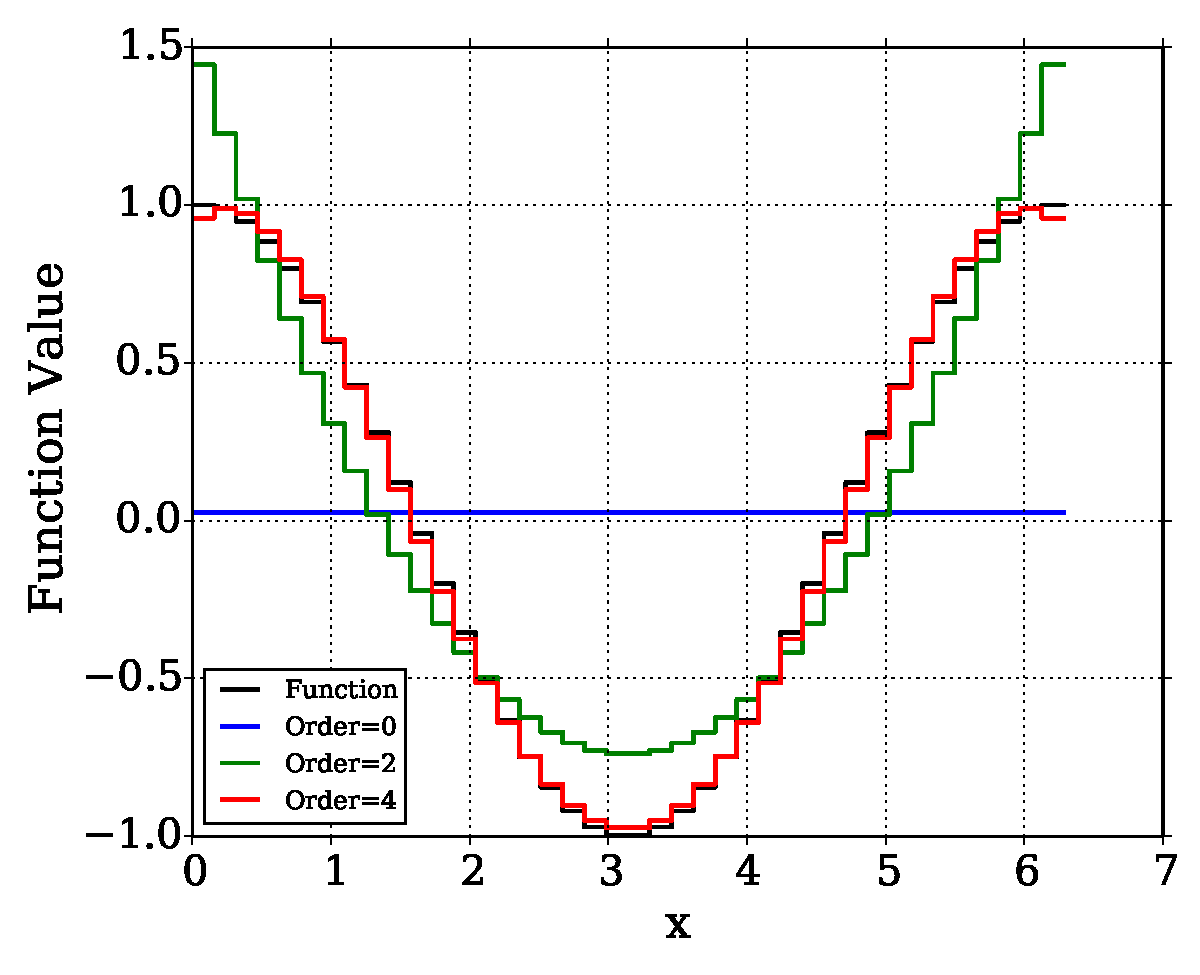
\includegraphics[trim=.1cm .25cm .1cm .4cm, clip=true,
    totalheight=0.35\textheight]{Figures/expansion}
    \caption{Using 40 discrete points, $\cos(x)\,  x\in[0,2\pi]$ expanded by 
Discrete Legendre Polynomials to $4^{th}$ order}
    \label{fig:DLPexpansion}
\end{figure*}

%-------------------------------------------------------------------------------

\section{Modified Discrete Legendre Polynomials}

To improve the DLPs as a basis for energy expansion, the polynomials are first 
modified by superimposing a ``shape'' vector $s$ on each basis vector, leading 
to the intermediate vectors
\begin{equation}
    \tilde{P}^h_{\text{mDLP}}(g) =  
    P^h_{\text{DLP}}(g) s(g) \,, \quad g = 1,\, 2,\, \ldots ,\, G \, .
\end{equation}
The modified Discrete Legendre Polynomial (mDLP) vectors  $P^h_{\text{mDLP}}$ 
are subsequently found by orthonormalizing the vectors 
$\tilde{P}^h_{\text{mDLP}}$. This formulation is referred to as Type 1 mDLP 
(mDLP-1) \citep{Roberts2014}. It is obvious that to expand a known 
function using the mDLP-1 basis, the best shape vector would be the function 
itself.  The power of 
modifying the DLP vectors is observed when using the same basis set to expand 
several different but related functions, e.g., the scalar flux as a function 
of energy for different spatial cells in a test problem.

As an example of mDLPs, consider a 10-pin test problem consisting of 5 pins of 
UO$_2$ next to 5 pins of mixed oxide (MOX), i.e., plutonium-bearing, fuel with 
reflective boundary 
conditions (this example problem is the first 1-D test problem discussed in 
\CHAPTER{Chapter4} and is shown in \FIG{fig:10-pin_config}).  This 
problem can be discretized spatially into several regions, i.e., N spatial 
cells.  Then the scalar flux $\phi$ can be calculated for 
each spatial cell, which leads to G group-dependent vectors that represent the 
scalar flux in each spatial cell.  In this case, a shape 
vector representing the spatially-averaged scalar flux as a function of energy 
is used to modify the DLP vectors and form the mDLP basis. This example shape 
vector is shown in \FIG{fig:shape_vec}.

\begin{figure*}[bt]
    \centering
    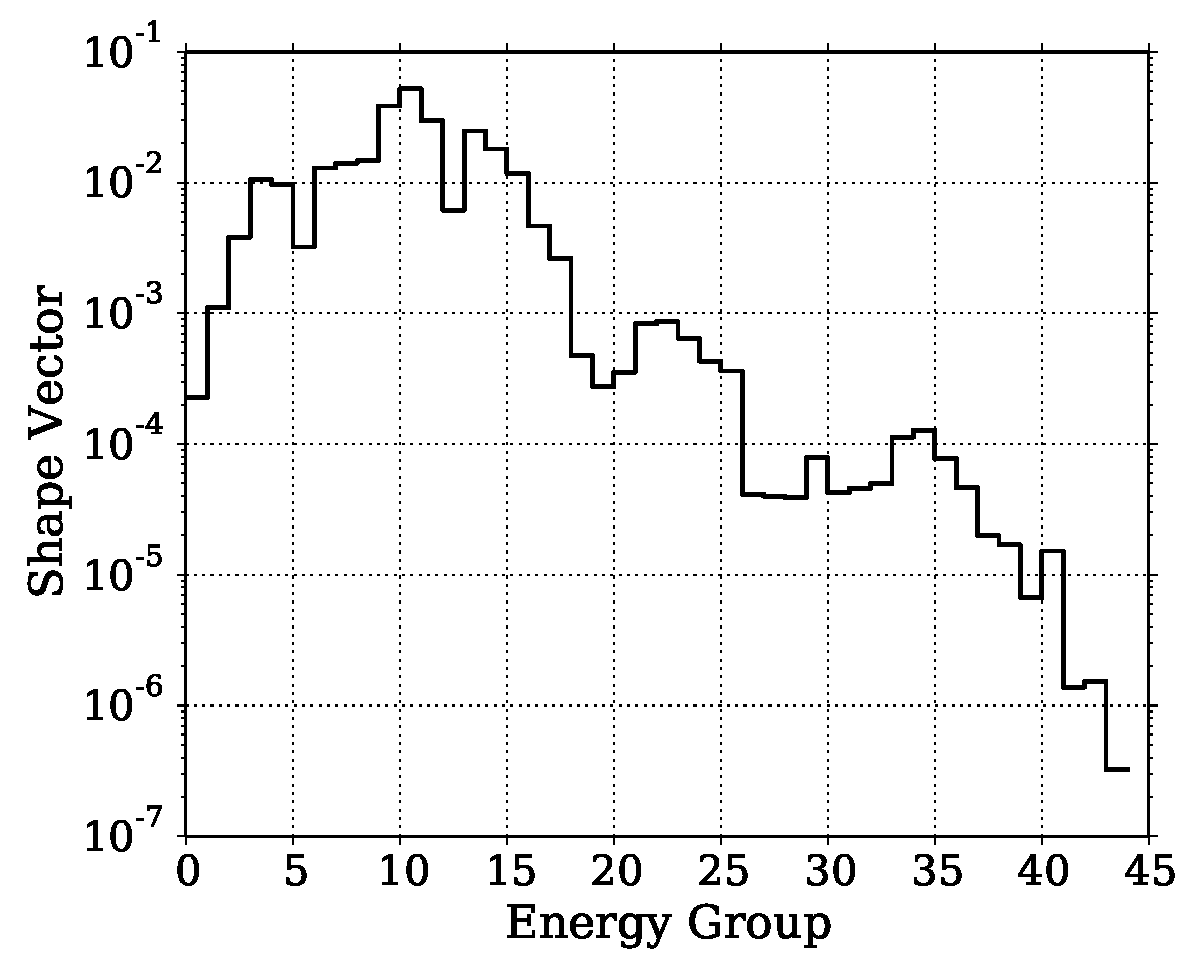
\includegraphics[trim=.1cm .25cm .1cm .35cm, clip=true,
    totalheight=0.35\textheight]{Figures/shape}
    \caption{Example shape vector for creating mDLP basis functions}
    \label{fig:shape_vec}
\end{figure*}

This shape vector will create the basis functions shown in \FIG{fig:mDLP} 
when using mDLP-1.  A second type of mDLP (mDLP-2) is formed by  
multiplying only the 
first DLP vector (i.e., the flat vector) with the shape function, 
then orthonormalizing the set of vectors \citep{Roberts2014}.  A sample of 
mDLP-2 
basis vectors is shown in \FIG{fig:mDLP2}.

\begin{figure*}[bt]
    \centering
    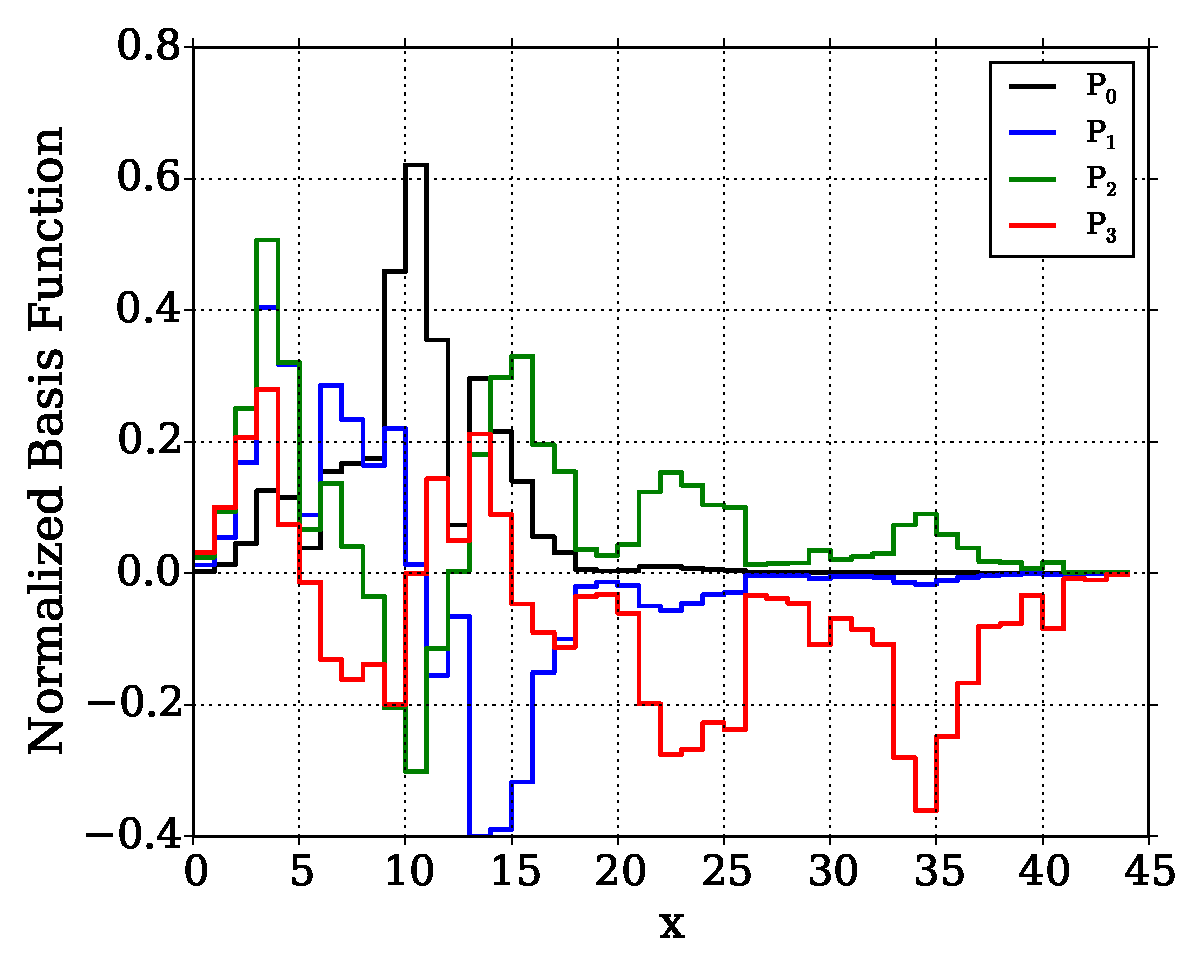
\includegraphics[trim=.1cm .25cm .1cm .4cm, clip=true,
    totalheight=0.35\textheight]{Figures/mDLP1_L_basis}
    \caption{Example basis functions for mDLP-1 shown through $3^{rd}$ 
        order}
    \label{fig:mDLP}
\end{figure*}

\begin{figure*}[bt]
    \centering
    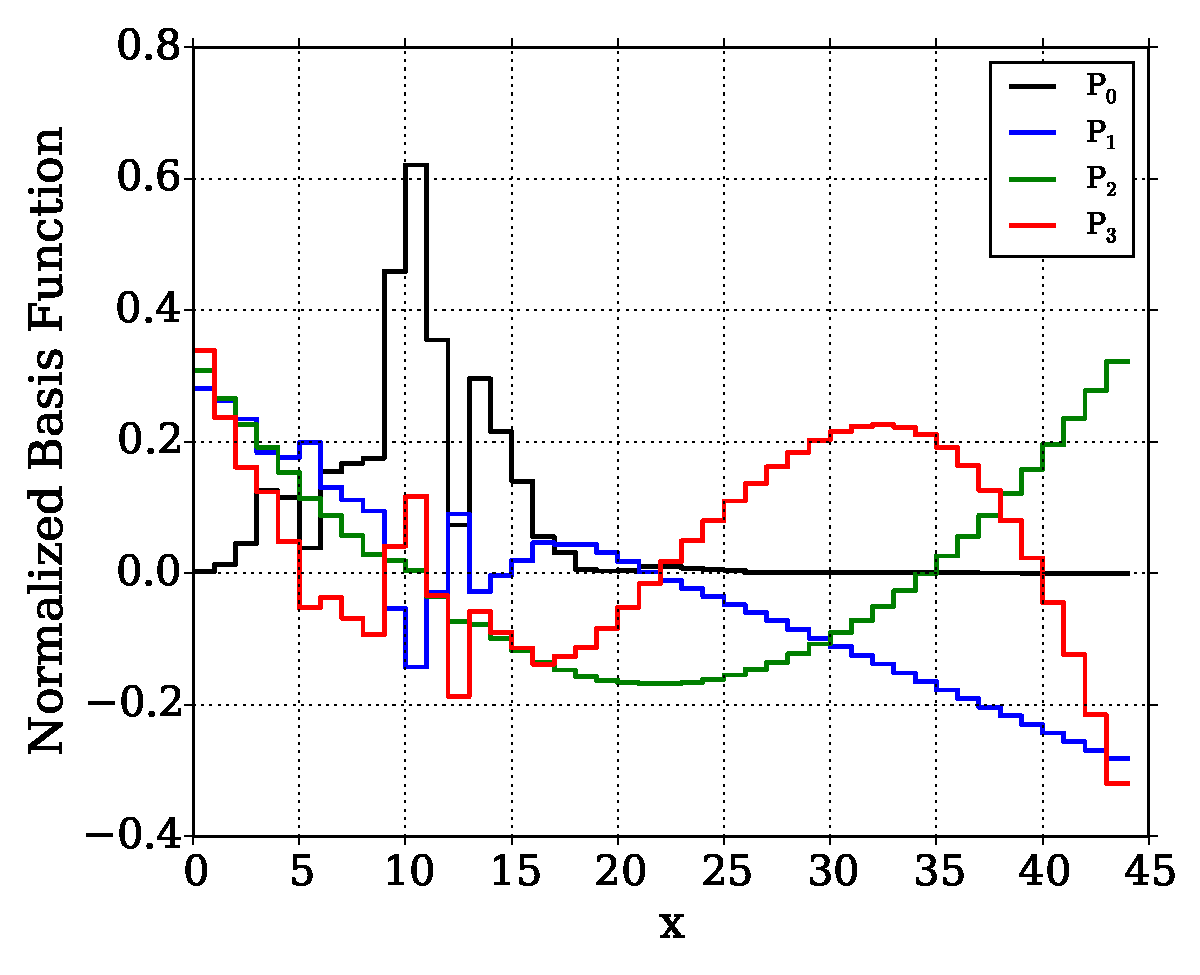
\includegraphics[trim=.1cm .25cm .1cm .4cm, clip=true,
    totalheight=0.35\textheight]{Figures/mDLP2_L_basis}
    \caption{Example basis functions for mDLP-2 shown through $3^{rd}$ 
        order}
    \label{fig:mDLP2}
\end{figure*}

The efficiency of the mDLP vectors are shown by computing the error due to 
expansion as a function of order.  The error is computed as
\begin{equation}
    \epsilon = \sqrt{\frac{\sum_{h=1}^H (f(h) - \tilde{f}(h))^2}{\sum_{h=1}^H
            f(h)^2}} \, ,
    \label{eq:l2norm}
\end{equation}
where $\tilde{f}(h)$ is the $h$th element of the approximate function $\tilde{f}$ as defined in 
\EQ{eq:expansion}. \EQUATION{eq:l2norm} is the discrete definition of 
the $L_2$ norm, which measures the deviation between two vectors in a least 
squares sense. \FIGURE{fig:mDLP expansion} shows the 
performance of both types of mDLP compared to DLP when used to expand the set 
of scalar flux vectors described for the example 10-pin case.  Note that at 
the full order (order = 43 for this example), all of the basis sets converge 
to within machine precision. It is clear that 
mDLP-1 outperforms mDLP-2, which suggests that more of the physics of the problem 
is captured by the lower-order functions of mDLP-1.  Thus, for this problem, the 
functions of mDLP-1 can better approximate the solution to the problem than 
mDLP-2. 

\begin{figure*}[bt]
    \centering
    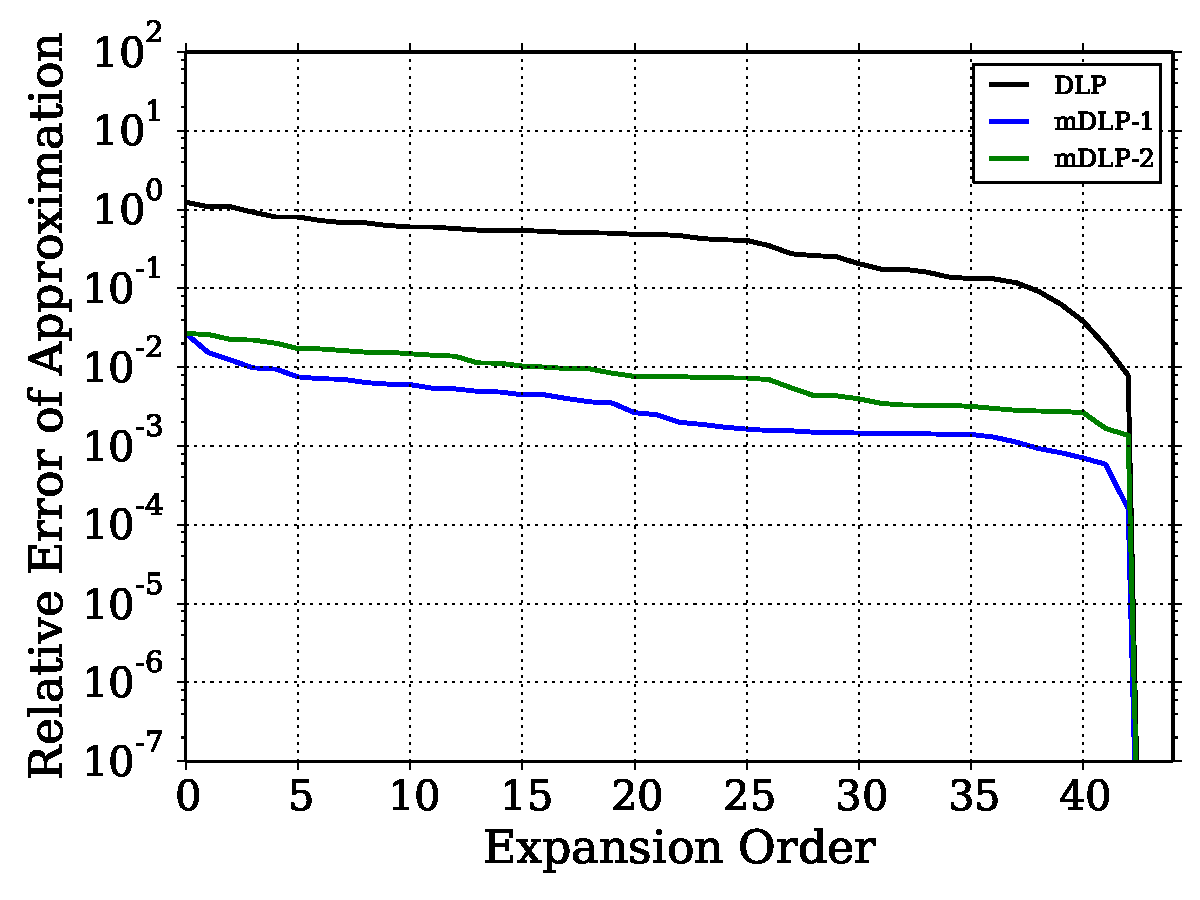
\includegraphics[trim=.1cm .25cm .1cm .32cm, clip=true,
    totalheight=0.35\textheight]{Figures/error_plot_f}
    \caption{Relative error in the $L_2$ norm as a function of expansion order 
for 
various basis 
        sets}
    \label{fig:mDLP expansion}
\end{figure*}

It must be reiterated that the solution for this problem was already known, and 
the shape 
vector was taken to be the average of the group-dependent vectors from each 
spatial cell.  In practice, the scalar flux will not be known {\it a priori}, 
thus a representative 
shape vector must be chosen.  For the 10-pin example in this chapter, 
a suitable shape vector may be constructed by taking the average of the spectrum 
produced by solving each type of fuel pin individually.  Although this 
approach is expected to produce a viable shape vector, the constructed 
basis set will not lead to the same accuracy as achieved when using the average 
of the actual spectra as the shape vector.

\section{Summary}

Later in Chapters \ref{Chapter5} and \ref{Chapter6}, DLP and mDLP are compared 
to the KLT (Karhunen-Lo\'{e}ve Transform) approach (which is discussed in 
\CHAPTER{Chapter3}).  The best case of mDLP (i.e., mDLP-1) is compared to 
each of the various formulations of the KLT.  However, the best-case mDLP 
requires the correct solution {\it a priori}.  A more practical 
use of 
mDLP is not expected to perform as well.  The best case mDLP was chosen as the 
comparison to provide a view into the performance of the KLT as used for basis 
generation.